\appendix
\setcounter{equation}{0}
\setcounter{figure}{0}
\renewcommand{\theequation}{A.\arabic{equation}}
\renewcommand\thefigure{A.\arabic{figure}}

\section{Online appendix}
\label{sec:Appendix}

This is the Online Appendix for the paper:

\begin{center}
Rodríguez-Sánchez P, van Nes EH, Scheffer M. \textit{Neutral competition boosts chaos in food webs}.
\end{center}

\subsection{Extra figures}
\label{subsec:ExtraFigures}

\subsubsection{Multispecies predator-prey network}
\label{subsubsec:MultispeciesPPNetwork}
\begin{figure}[H]
	\begin{center}
		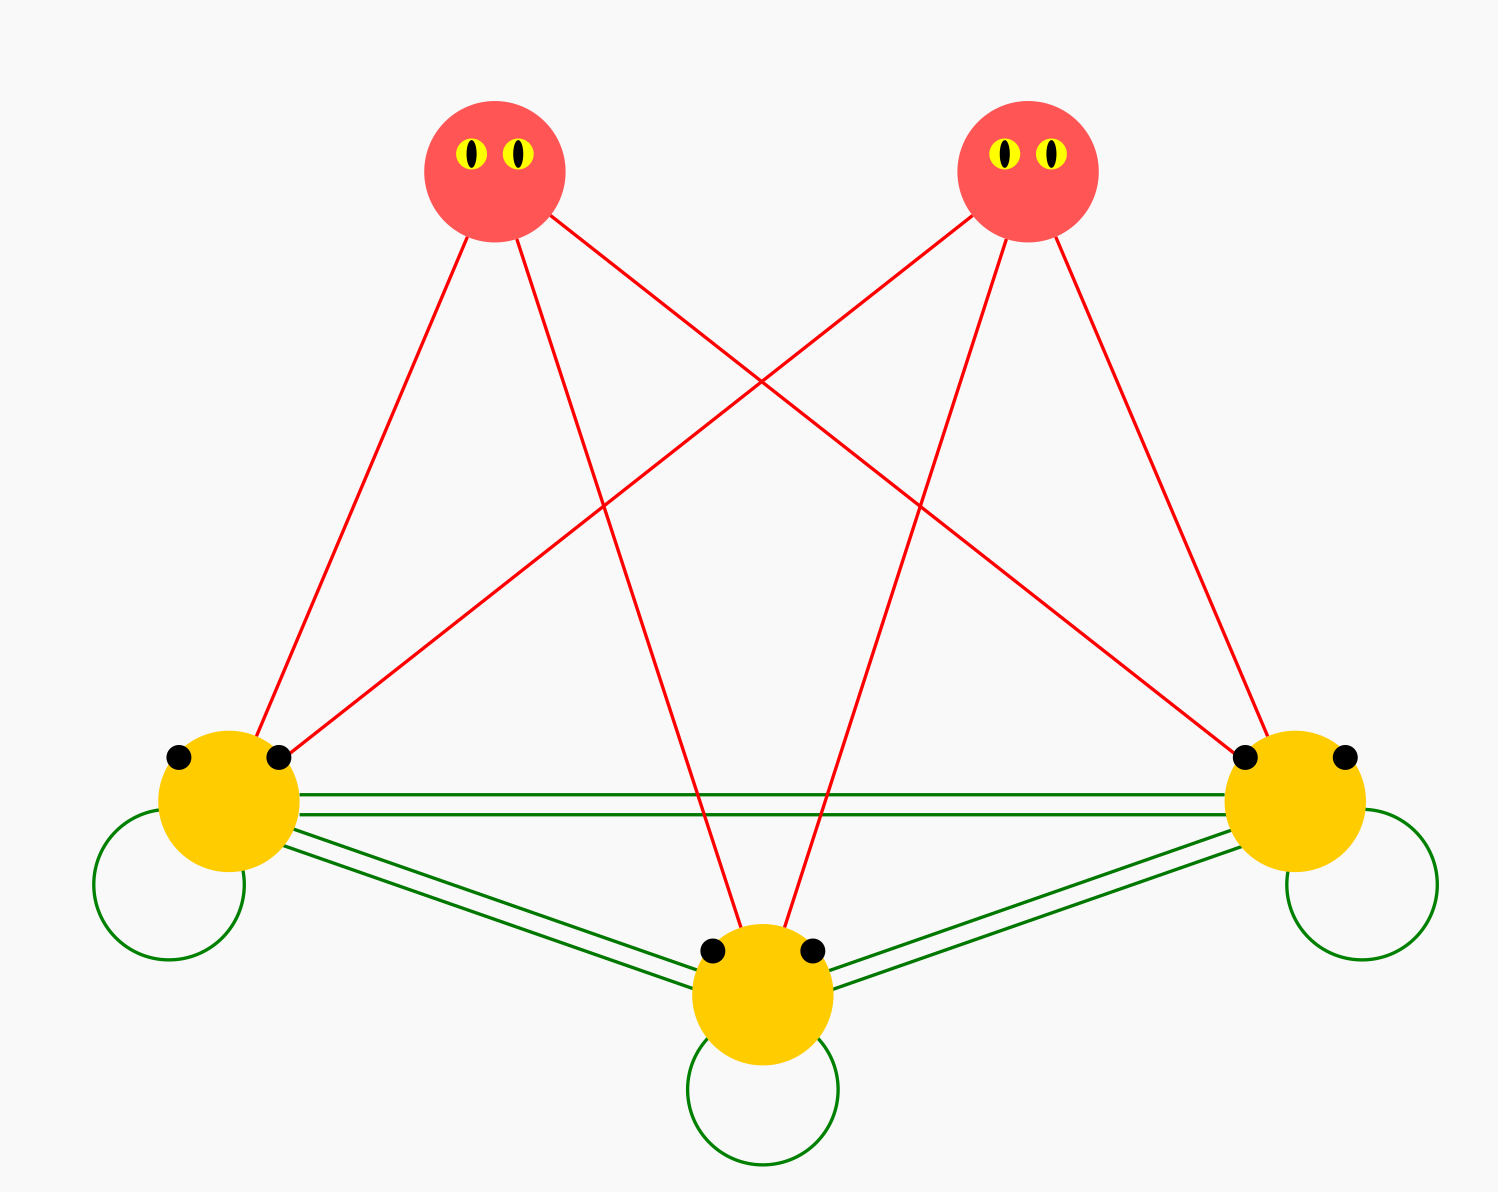
\includegraphics[width=0.5\columnwidth]{net.png}
	\end{center}
	\caption{Example with $2$ consumers and $3$ prey. Each one of the red links represents a predation interaction (coded in the matrix of predator preference coefficients, $ S $). Each green link represents a competition interaction (coded in the matrix of competition coefficients, $ A $). The closed green loops are related with carrying capacity (diagonal elements of $ A $) interpreted here as intra-species competition.}
	\label{fig:Network}
\end{figure}

\subsubsection{Probabilities grouped by number of species}
\label{subsubsec:AllProbabilities}
\begin{figure}[H]
	\begin{center}
		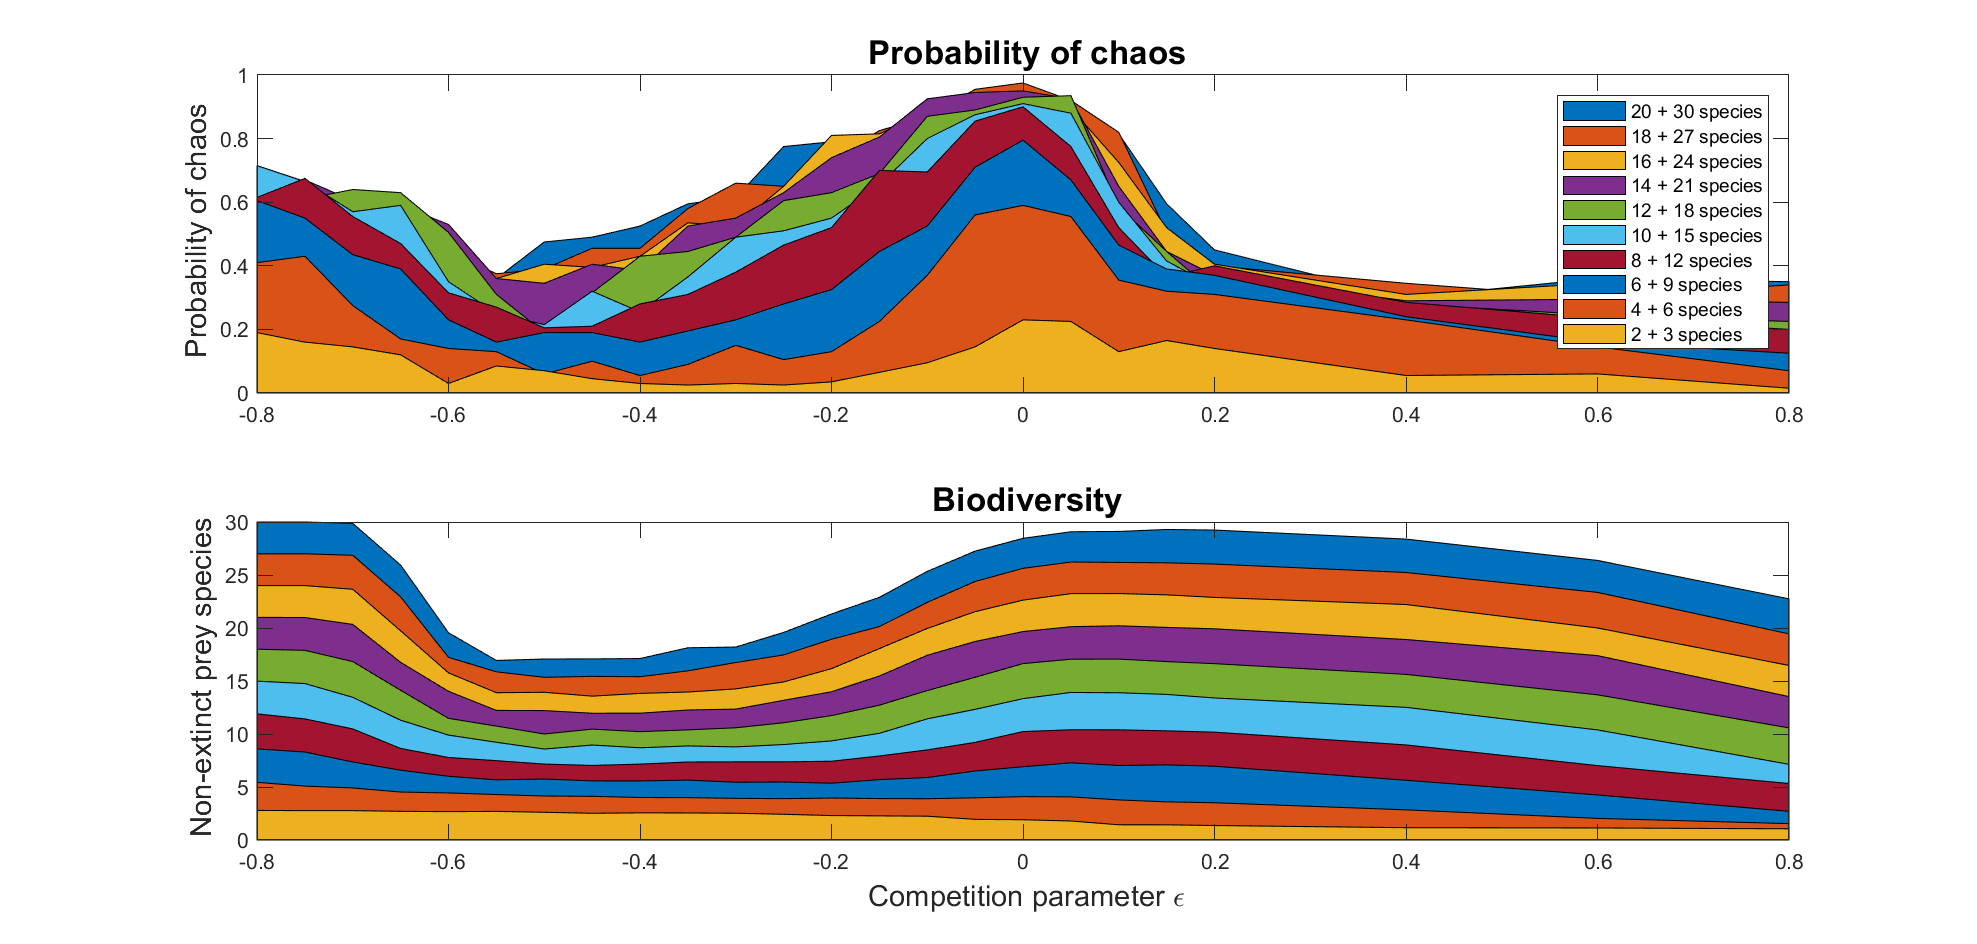
\includegraphics[width=1\columnwidth]{results_all.png}
	\end{center}
	\caption{Summary of the results of the whole set of simulations. The competition parameter $\epsilon$ is on the horizontal axis. The estimated probability of chaos is represented on the vertical one. Each panel corresponds to an ecosystem with a different number of interacting species. The exact number is shown in each box, as number of predators + number of prey.}
	\label{fig:AllProbabilities}
\end{figure}

\subsubsection{Biodiversity measurements}
\label{subsubsec:BiodiversityFigs}

For each simulation, a biodiversity index was estimated as the number of prey species whose population was higher than a minimum threshold of $\bioThreshold$ $mg$ $l^{-1}$, averaged respective to time.

\begin{figure}[H]
	\begin{center}
		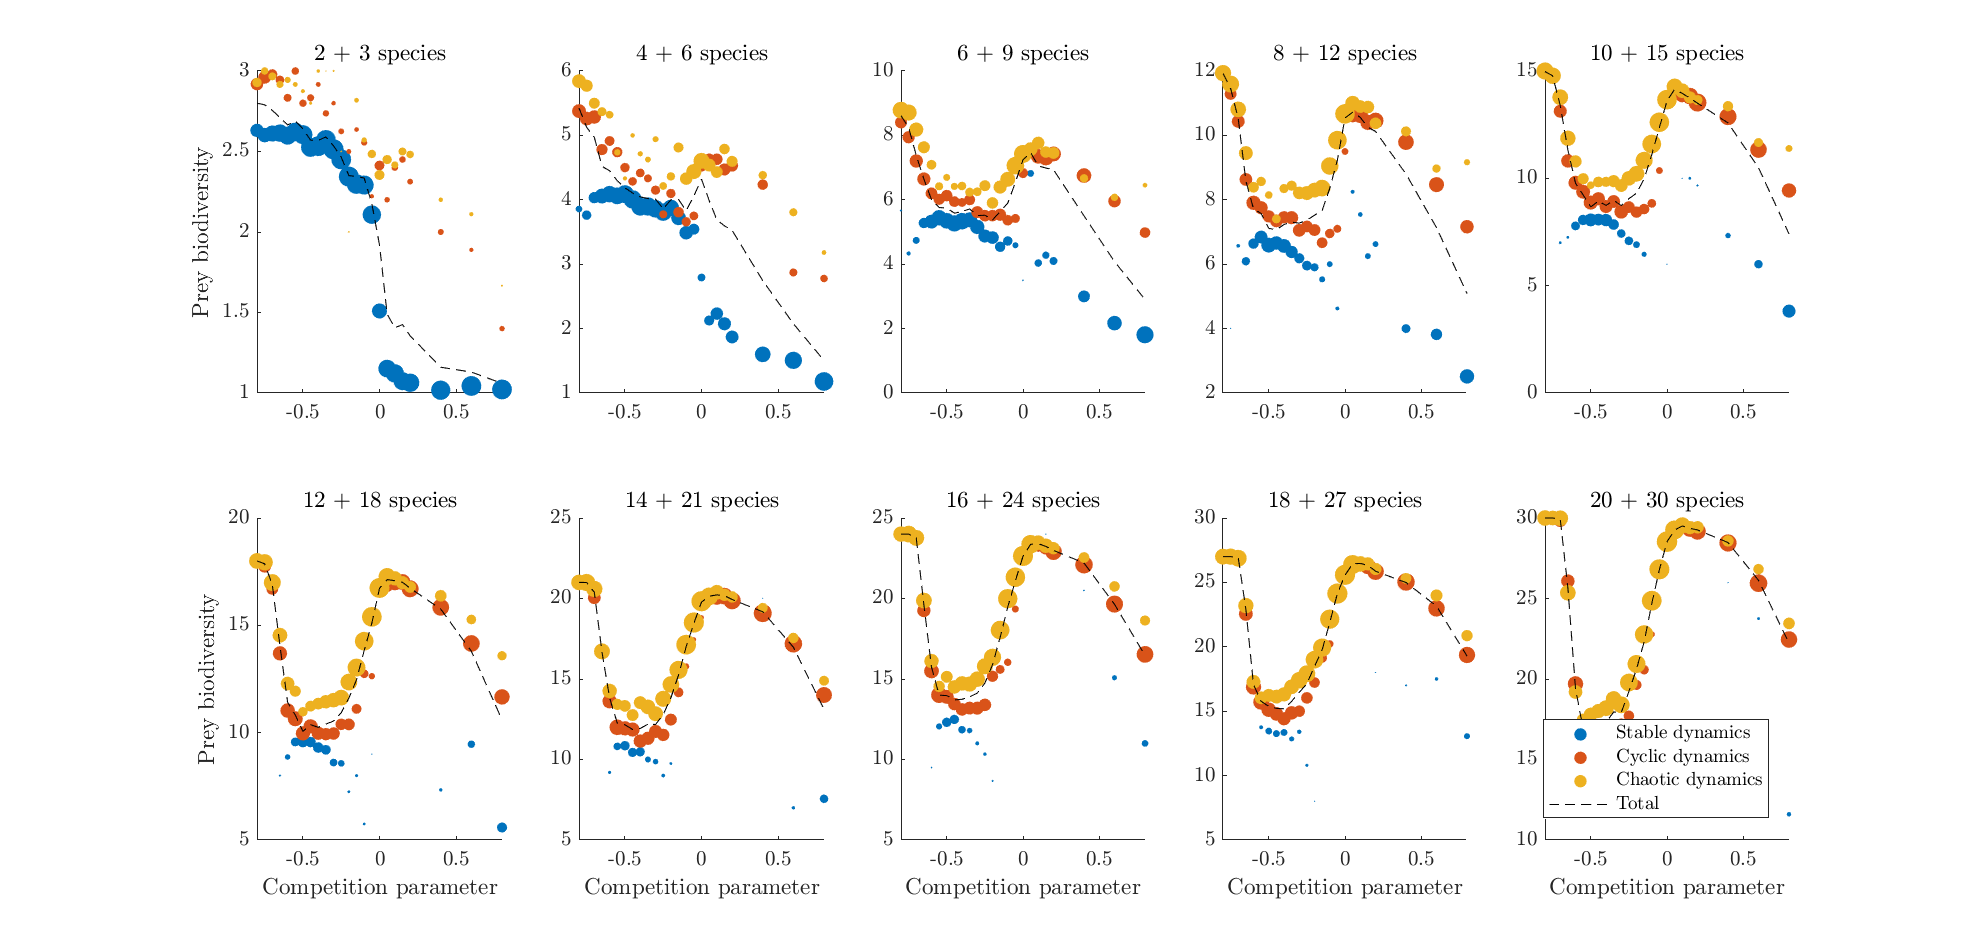
\includegraphics[width=1\columnwidth]{biod_split_by_dynamics.png}
	\end{center}
	\caption{Average prey biodiversity vs. competition parameter. Each panel shows a food network of a different size. For each value of the competition parameter, 200 randomly drawn ecosystems were simulated. The dashed line shows the average number of prey species of these 200 simulations. The white circles represent the average prey biodiversity of those simulations who had chaotic dynamics, the black circles represent the same for non-chaotic dynamics. The relative area of the white to the black circles represents the ratio of chaotic to regular dynamics.}
	\label{fig:BiodSplitByChaos}
\end{figure}

\begin{figure}[H]
	\begin{center}
		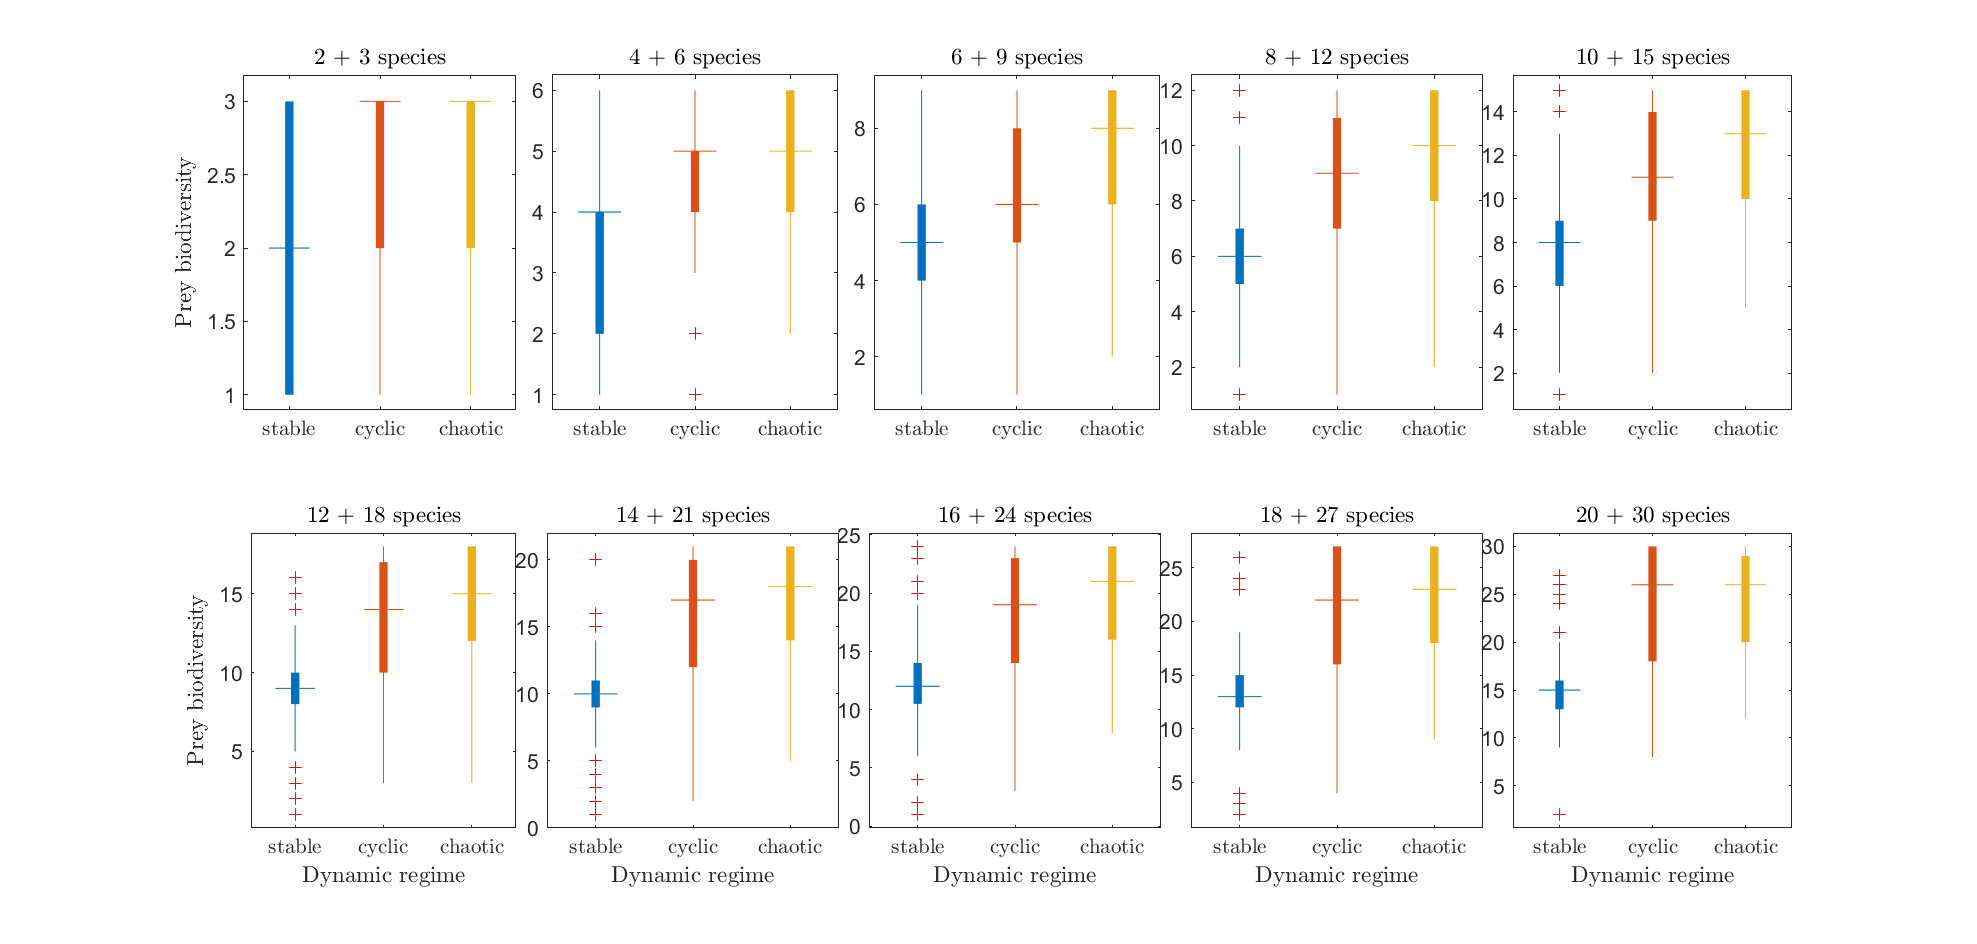
\includegraphics[width=1\columnwidth]{biod_box_and_whisker.png}
	\end{center}
	\caption{Box and whisker plot of the prey biodiversity, after being classified as regular or chaotic.}
	\label{fig:BiodBoxAndWhisker}
\end{figure}

\begin{figure}[H]
	\begin{center}
		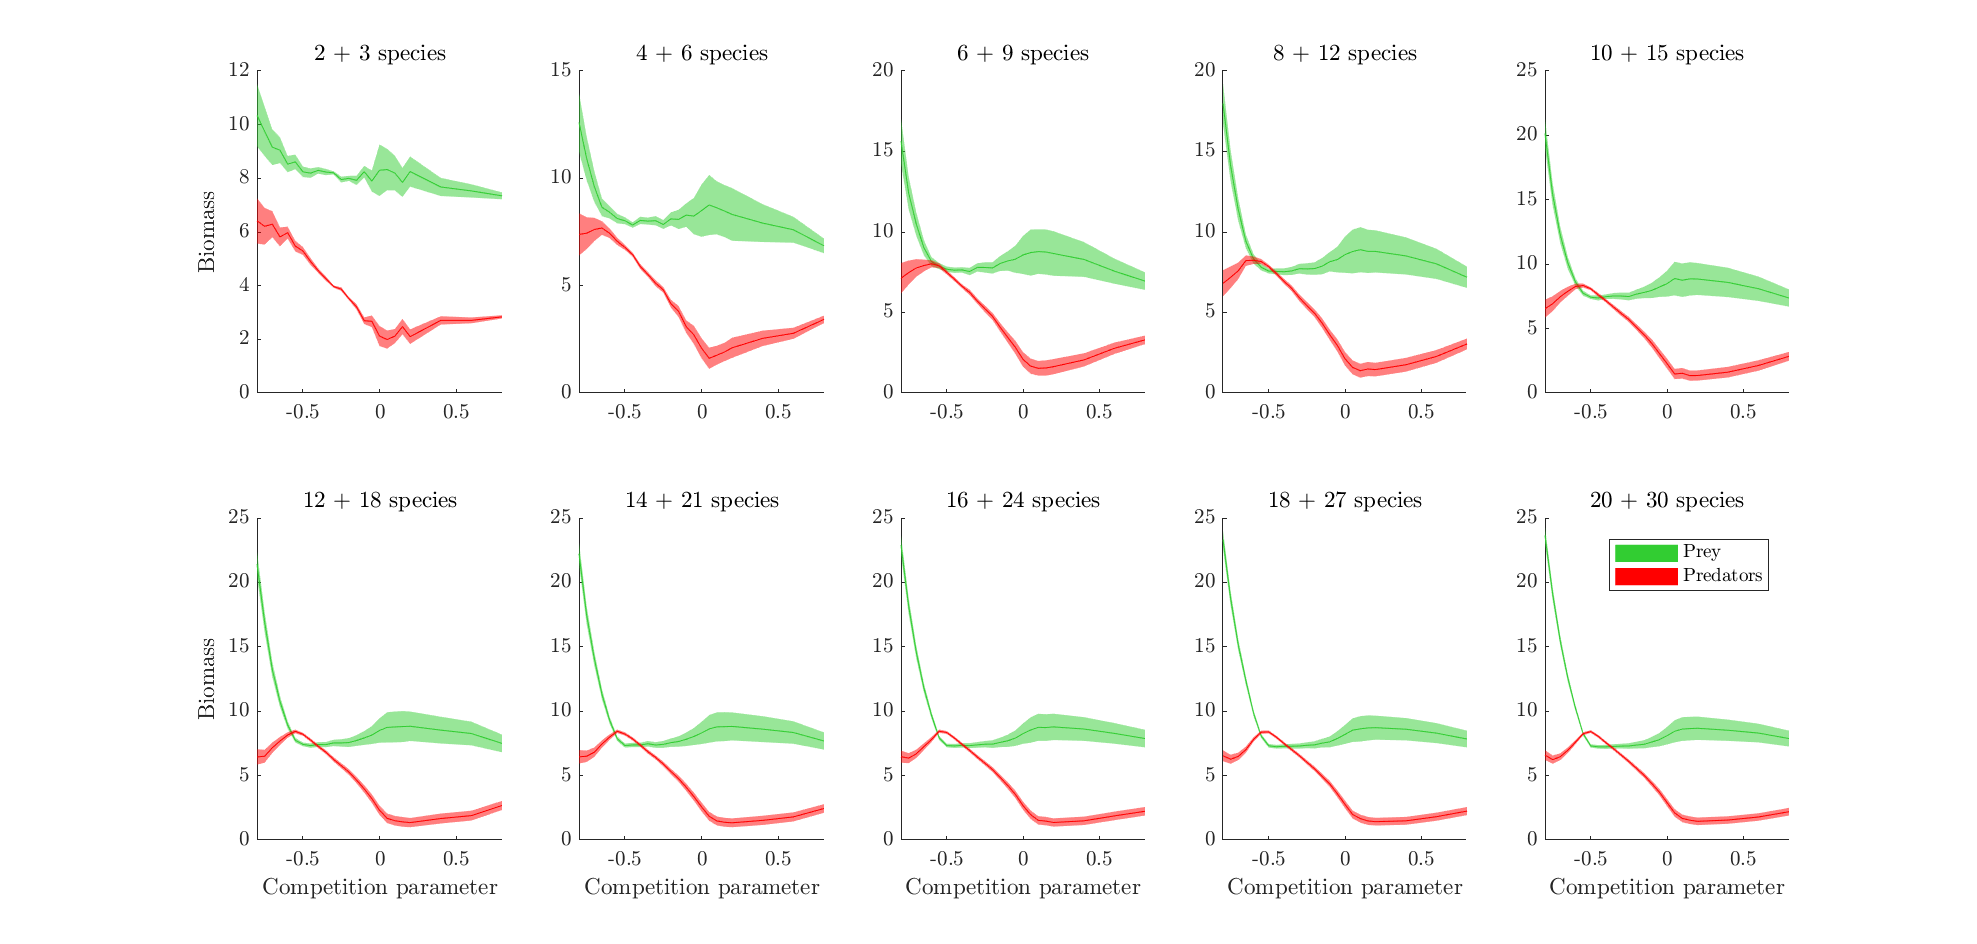
\includegraphics[width=1\columnwidth]{biomass.png}
	\end{center}
	\caption{Average biomasses grouped by trophic level vs. competition parameter. The width represents standard deviation.}
	\label{fig:Biomass}
\end{figure}

\subsubsection{Flow chart}
\label{subsubsec:FlowChart}
In the spirit of reproducible research we made available all the analysis code used to draw our conclusions. Any interested researcher can clone it from a \textit{GitHub} repository \citep{Rodriguez-Sanchez-code-neuchaos} and, executing a single script, reproduce all our simulations and figures. This figure shows schematically what this script does:

\begin{figure}[H]
	\begin{center}
		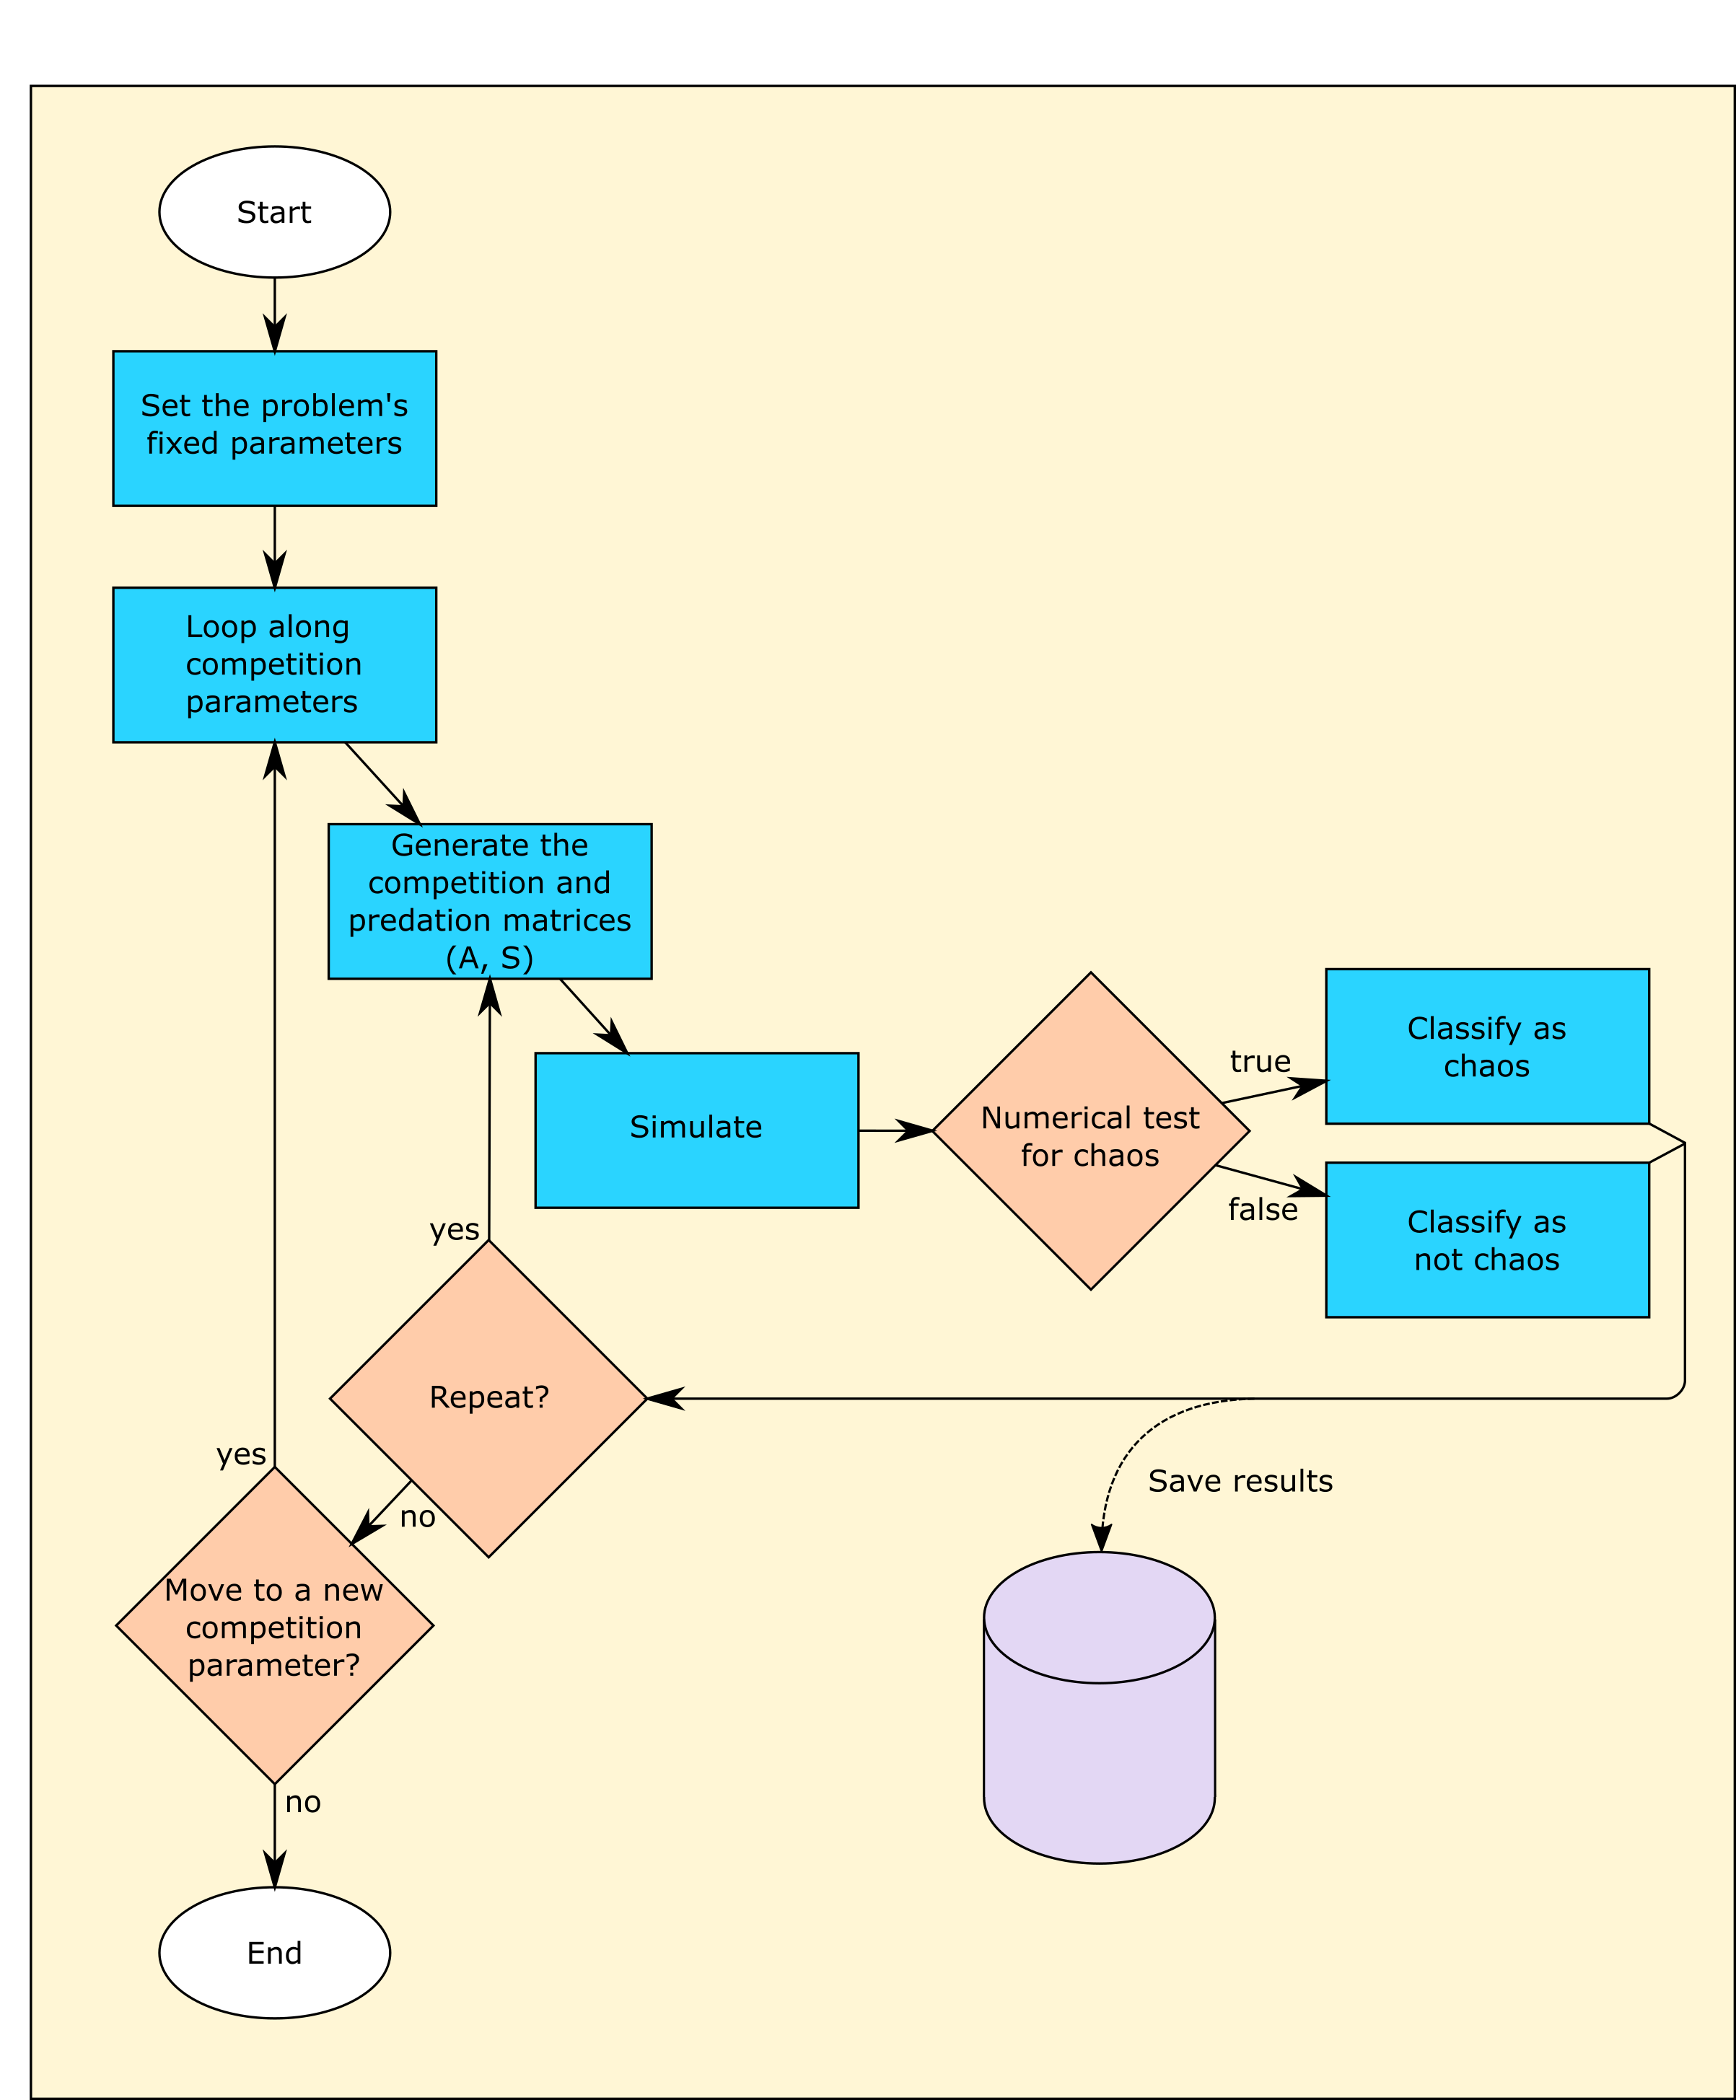
\includegraphics[width=0.8\columnwidth]{flow_chart.png}
	\end{center}
	\caption{Flow chart describing the numerical experiment. The source code is available at \textit{\texttt{https://doi.org/10.5281/zenodo.1319590}}.}
	\label{fig:FlowChart}
\end{figure}
